\documentclass[14pt]{extarticle}
\usepackage[english,ukrainian]{babel}
\usepackage[utf8]{inputenc}
\usepackage{amsmath,amssymb}
\usepackage{parskip}
\usepackage{graphicx}
\usepackage{xcolor}
\usepackage{tcolorbox}
\tcbuselibrary{skins}
\usepackage[framemethod=tikz]{mdframed}
\usepackage{chngcntr}
\usepackage{enumitem}
\usepackage{hyperref}
\usepackage{float}
\usepackage{subfig}
\usepackage{esint}
\usepackage[top=2.5cm, left=3cm, right=3cm, bottom=4.0cm]{geometry}
\usepackage[table]{xcolor}
\usepackage{algorithm}
\usepackage{algpseudocode}
\usepackage{listings}

\tcbuselibrary{theorems}

\newtcbtheorem[number within=section]{statement}{Твердження}%
{colback=blue!5,colframe=blue!35!black,fonttitle=\bfseries}{th}

\title{Домашня робота з курсу ``Теорія Ймовірності''}
\author{Студента 3 курсу групи МП-31 Захарова Дмитра}
\date{\today}

\begin{document}

\maketitle

\section*{Завдання 1.} 

\textbf{Умова.} Через кожну годину вимірювалась напруга в електромережі. Результати вимірювання напруги:
\begin{gather*}
\mathcal{X}=\{222, 219, 224, 220, 218, 217, 221, 220, 215, 218, 223, 225,\\ 220, 226, 221, 216, 211, 219, 220, 221, 222, 218, 221, 219\}
\end{gather*}
Побудувати вибіркову функцію розподілу, знайти вибіркове середнє, вибіркову дисперсію та незміщенну оцінку дисперсії.

\textbf{Розв'язок.} 

\textbf{Вибіркова функція розподілу.} Спочатку відсортуємо елементи послідовності $\mathcal{X}$:
\begin{gather*}
\mathcal{X}' = \{211, 215, 216, 217, 218, 218, 218, 219, 219, 219, \\ 220, 220, 220, 220, 221, 221, 221, 221, 222, 222, 223, 224, 225, 226\}
\end{gather*}

Позначимо через $m$ кількість різних елементів $\mathcal{X}'$. За означенням, вибіркова функція розподілу:
\[
\hat{F}_n(x) = \begin{cases}
    0, & x \leq \mathcal{X}'_1 \\
    \sum_{j=1}^i\frac{\nu_j}{n}, & x \in (\mathcal{X}'_i, \mathcal{X}'_{i+1}], \; i\in \{1,\dots,m-1\} \\
    1, & x > \mathcal{X}_{m}
\end{cases},
\]
де $\mathcal{X}'_i$ це значення $i$-ого унікального значення за порядком зростання, а $\nu_j$ є частотою появи цього значення.  

В нашому випадку маємо
\begin{gather*}
\mathcal{X}'_1=211, \; \nu_1 = 1 \\
\mathcal{X}'_2=215, \; \nu_2 = 1 \\
\mathcal{X}'_3=216, \; \nu_3 = 1 \\
\mathcal{X}'_4=217, \; \nu_4 = 1 \\
\mathcal{X}'_5=218, \; \nu_5 = 3 \\
\mathcal{X}'_6=219, \; \nu_6 = 3 \\
\mathcal{X}'_7=220, \; \nu_7 = 4 \\
\mathcal{X}'_8=221, \; \nu_8 = 4 \\
\mathcal{X}'_9=222, \; \nu_9 = 2 \\
\mathcal{X}'_{10}=223, \; \nu_{10} = 1 \\
\mathcal{X}'_{11}=224, \; \nu_{11} = 1 \\
\mathcal{X}'_{12}=225, \; \nu_{12} = 1 \\
\mathcal{X}'_{13}=226, \; \nu_{13} = 1 \\
\end{gather*}

Отже,
\[
\hat{F}_n(x) = \begin{cases}
    0, & x \leq 211 \\
    \frac{1}{24}, & 211 < x \leq 215 \\
    \frac{2}{24}, & 215 < x \leq 216 \\
    \frac{3}{24}, & 216 < x \leq 217 \\
    \frac{4}{24}, & 217 < x \leq 218 \\
    \frac{7}{24}, & 218 < x \leq 219 \\
    \frac{10}{24}, & 219 < x \leq 220 \\
    \frac{14}{24}, & 220 < x \leq 221 \\
    \frac{18}{24}, & 221 < x \leq 222 \\
    \frac{20}{24}, & 222 < x \leq 223 \\
    \frac{21}{24}, & 223 < x \leq 224 \\
    \frac{22}{24}, & 224 < x \leq 225 \\
    \frac{23}{24}, & 225 < x \leq 226 \\
    1, & x > 226
\end{cases}
\]

\textbf{Вибіркове середнє.} Згідно означенню,
\[
\overline{\mu} = \frac{1}{n}\sum_{x \in \mathcal{X}} x \approx 219.83
\]
Вибіркова дисперсія:
\begin{gather*}
\overline{\sigma}^2 = \frac{1}{n}\sum_{i=1}^k \mathcal{X}'_i^2\nu_i- \overline{\mu}^2 \approx 10.14 \implies \overline{\sigma}\approx 3.18
\end{gather*}
Незміщена оцінка дисперсії:
\begin{gather*}
    \hat{\sigma}^2 = \frac{n}{n-1}\cdot\overline{\sigma}^2 = \frac{24}{23}\overline{\sigma}^2 \approx 10.58 \implies \hat{\sigma} \approx 3.25
\end{gather*}

\pagebreak
\section*{Завдання 2.}
\textbf{Умова.} Нижче наведені дані про час, витрачений робочими на виготовлення
однієї деталі. Побудувати вибіркову функцію розподілу, гістограму
вибірки та полігон частот. Знайти вибіркове середнє, вибіркову
дисперсію і незміщену оцінку дисперсії.
\begin{center}
\begin{tabular}{ |c|c|c|c|c|c| } 
\hline
\textbf{Інтервали часу, хвил.} & [4.0,4.4) & [4.4,4.8) & [4.8,5.2) & [5.2,5.6) & [5.6,6.0) \\ \hline
\textbf{Кількість робочих} & 5 & 8 & 21 & 31 & 19 \\ \hline
\end{tabular}
\end{center}

\textbf{Розв'язок.} Замінуємо інтервали на середини інтервалів і отримуємо вибірку зі значень $\{4.2,4.6,5.0,5.4,5.8\}$ з відповідними частотами $\{5,8,21,31,19\}$. Сумарна кількість елементів $84$. Отже, вибіркова функція:
\[
\hat{F}_n(x) = \begin{cases}
    0, & x \leq 4.2\\
    \frac{5}{84}, & 4.2 < x \leq 4.6 \\
    \frac{13}{84}, & 4.6 < x \leq 5.0 \\
    \frac{34}{84}, & 5.0 < x \leq 5.4 \\
    \frac{65}{84}, & 5.4 < x \leq 5.8 \\
    1, & x > 5.8
\end{cases}
\]
Гістограма вибірки зображена на рис. \ref{fig:1}.
\begin{figure}[H]
    \centering
    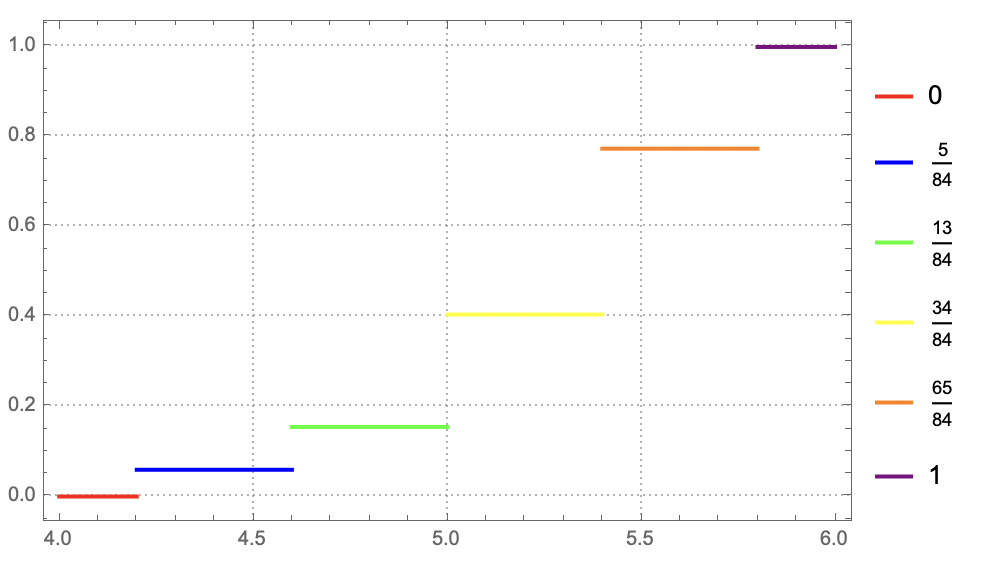
\includegraphics[width=0.7\textwidth]{images/hw_11/histogram.png}
    \caption{Гістограма вибірки}
    \label{fig:1}
\end{figure}

Вибіркове середнє:
\[
\overline{\mu} = \frac{1}{n}\sum_{i=1}^n \nu_i y_i \approx 5.243
\]
Вибіркова дисперсія:
\[
\overline{\sigma}^2 = \frac{1}{n}\sum_{i=1}^n \nu_i y_i^2 - \overline{\mu}^2 \approx 0.198 \implies \overline{\sigma} \approx 0.445
\]
Незміщена оцінка:
\[
\hat{\sigma} = \frac{n}{n-1} \cdot \overline{\sigma}^2 \approx 0.2 \implies \hat{\sigma} \approx 0.448
\]

\pagebreak
\section*{Завдання 3.}

\textbf{Умова.} Знайти за методом максимальної правдоподібності оцінку параметру $\theta$ біноміального закону розподілу, якщо $N$ -- відоме:
\[
p(X=k \mid \theta) = C_N^k\theta^k(1-\theta)^k, \; k \in \{0,\dots,N\}
\]

\textbf{Розв'язок.} Нехай маємо вибірку $X=\{x_1,x_2,\dots,x_n\} \sim \text{Bin}(N,\theta)$. За означенням:
\[
\hat{\theta}_{\text{MLE}} \triangleq \arg\max_{\theta} p(X \mid \theta)
\]
Функція правдоподібності:
\[
p(X \mid \theta) = \prod_{i=1}^n p(X=x_i;\theta)
\]
Отже, маємо:
\[
\hat{\theta}_{\text{MLE}} = \arg\max_{\theta} \prod_{i=1}^n C_N^{x_i} \theta^{x_i}(1-\theta)^{x_i} = N! \cdot \arg\max_{\theta}\prod_{i=1}^n \frac{\theta^{x_i}(1-\theta)^{x_i}}{x_i!(N-x_i)!}
\]
Тепер нам легше оптимізовувати логарифм виразу під максимумом:
\begin{gather*}
\hat{\theta}_{\text{MLE}} = \arg\max_{\theta}\log\prod_{i=1}^n \frac{\theta^{x_i}(1-\theta)^{x_i}}{x_i!(N-x_i)!} = \arg\max_{\theta}\sum_{i=1}^n \log \frac{\theta^{x_i}(1-\theta)^{x_i}}{x_i!(N-x_i)!} \\
= \arg\max_{\theta} \sum_{i=1}^n \left\{ \log \theta^{x_i}(1-\theta)^{x_i} - \log x_i!(N-x_i)!\right\} \\
= \arg\max_{\theta} \left(\sum_{i=1}^n \left\{x_i\log\theta + x_i\log(1-\theta)\right\} - \sum_{i=1}^n \log x_i!(N-x_i)!\right)
\end{gather*}

Помітимо, що друга сума не залежить від $\theta$, тому
\begin{gather*}
\hat{\theta}_{\text{MLE}} = \arg\max_{\theta} \sum_{i=1}^n\left\{ x_i\log\theta + x_i \log(1-\theta)\right\}\\ = \arg\max_{\theta}\left(\log\theta \sum_{i=1}^n x_i + \log(1-\theta)\sum_{i=1}^n x_i\right) = n\overline{\mu}\arg\max_{\theta}(\log \theta + \log(1-\theta))
\end{gather*}

Бачимо, що можна прибрати $\sum_{i=1}^n x_i \equiv n\overline{\mu}$ з виразу для оптимізації і тоді залишається
\[
\hat{\theta}_{\text{MLE}} = \arg\max_{\theta} \log \theta(1-\theta) = \arg\max_{\theta} \theta(1-\theta) = \frac{1}{2}
\]

\textbf{Відповідь.} $\hat{\theta}_{\text{MLE}} = \frac{1}{2}$.

\section*{Завдання 4.}

\textbf{Умова.} Знайти методом максимальної правдоподібності оцінку параметру $\theta$ геометричного розподілу
\[
p(X=k\mid\theta) = \theta^k(1-\theta)
\]

\textbf{Розв'язок.} Нехай маємо вибірку $X=\{x_1,x_2,\dots,x_n\}$. Тоді:
\begin{gather*}
\hat{\theta}_{\text{MLE}} = \arg\max_{\theta} \prod_{i=1}^n p(X=x_i\mid \theta) = \arg\max_{\theta} \prod_{i=1}^n \theta^{x_i}(1-\theta) \\
= \arg\max_{\theta} \theta^{\sum_{i=1}^n x_i}(1-\theta)^n
\end{gather*}
Знову переходимо до логарифмів:
\[
\hat{\theta}_{\text{MLE}} = \arg\max_{\theta}\left(\log\theta\sum_{i=1}^n x_i + n\log(1-\theta)\right) = \arg\max_{\theta}\left(\overline{\mu}\log\theta + \log(1-\theta) \right),
\]
де ми позначили $\overline{\mu} := \frac{1}{n}\sum_{i=1}^n x_i$. Отже, треба оптимізувати функцію:
\[
f_{\overline{\mu}}(\theta) = \overline{\mu}\log\theta + \log(1-\theta)
\]
Знайдемо екстремум:
\[
\frac{\partial f_{\overline{\mu}}}{\partial \theta} = \frac{\overline{\mu}}{\theta} - \frac{1}{1-\theta} = 0 \implies \hat{\theta} = \frac{\overline{\mu}}{1+\overline{\mu}}
\]
\textbf{Відповідь.} $\hat{\theta}_{\text{MLE}} = \frac{\overline{\mu}}{1+\overline{\mu}}$ де $\overline{\mu}$ є вибірковим середнім. 

\section*{Вправа 1 (з лекції).}

\textbf{Умова.} 

\textit{Частина 1.} Доведіть наступну формулу для обчислення вибіркової дисперсії, яке зручно використовувати при її підрахунку
\[
\overline{\sigma}^2 = \frac{1}{n}\sum_{i=1}^n x_i^2 - \overline{\mu}^2
\]

\textit{Частина 2.} Доведіть наступне зображення для вибіркової дисперсії
\[
\overline{\sigma}^2 = \frac{1}{n}\sum_{i=1}^n (x_i-a)^2 - (\overline{\mu}-a)^2
\]
Чому цю формулу не можна зазвичай застосовувати на практиці при обчисленні вибіркової дисперсії?

\textbf{Доведення.} 

\textit{Частина 1.} За означенням, вибіркова дисперсія:
\[
\overline{\sigma}^2 \triangleq \frac{1}{n}\sum_{i=1}^n (x_i-\overline{\mu})^2
\]
Розпишемо цей вираз:
\begin{gather*}
\overline{\sigma}^2 = \frac{1}{n}\left(\sum_{i=1}^n x_i^2 - 2\sum_{i=1}^n x_i\overline{\mu} + \sum_{i=1}^n \overline{\mu}^2\right) \\
= \frac{1}{n}\left(\sum_{i=1}^n x_i^2 - 2\overline{\mu}\underbrace{\sum_{i=1}^nx_i}_{=n\overline{\mu}} + n\overline{\mu}^2\right) = \frac{1}{n}\sum_{i=1}^n x_i^2 - \overline{\mu}^2
\end{gather*}

Інший, меньш строгий спосіб полягає в тому, щоб помітити, що $\text{Var}[\xi] = \mathbb{E}[\xi^2]-\mathbb{E}[\xi]^2$, звідки одразу випливає початкове твердження (оскільки $\mathbb{E}[\xi^2]$ це середнє квадратів, а $\mathbb{E}[\xi]$ -- середнє у квадраті). 

\textit{Частина 2.}
\begin{gather*}
\frac{1}{n}\sum_{i=1}^n (x_i-a)^2 - (\overline{\mu}-a)^2 = \frac{1}{n}\sum_{i=1}^n x_i^2 - \frac{2a}{n}\underbrace{\sum_{i=1}^n x_i}_{=n\overline{\mu}} + \frac{a^2}{n} \cdot n - (\overline{\mu}-a)^2 \\
= \frac{1}{n}\sum_{i=1}^n x_i^2 - 2a\overline{\mu} + a^2 - \overline{\mu}^2 + 2a\overline{\mu} - a^2 = \frac{1}{n}\sum_{i=1}^n x_i^2 - \overline{\mu}^2 \triangleq \overline{\sigma}^2
\end{gather*}

В цілому, цю формулу напевно і можна використовувати, проте віднімання $a$ від усіх параметрів може зменшити точність самих розрахунків.

\section*{Вправа 2 (з лекції).}

\textbf{Умова.} Чому оцінка 
\[
\hat{\sigma}^2 = \frac{n}{n-1} \cdot \overline{\sigma}^2
\]
буде незміщеною оцінкою дисперсії?

\textbf{Розв'язок.} Як було доведено на лекції:
\[
\mathbb{E}[\overline{\sigma}^2] = \left(\frac{n-1}{n}\right)\sigma^2
\]
Отже:
\[
\mathbb{E}[\hat{\sigma}^2] = \frac{n}{n-1} \cdot \mathbb{E}[\overline{\sigma}^2] = \sigma^2,
\]
що за означенням є незміщеною оцінкою.

\section*{Вправа 3 (з лекції).} 

\textbf{Умова.} Доведіть, що $\overline{\mu}_1 = \frac{1}{n}\sum_{i=1}^n(x_i-\overline{\mu})=0$

\textbf{Розв'язок.} $\sum_{i=1}^n(x_i-\overline{\mu}) = \frac{1}{n}\sum_{i=1}^n-\overline{\mu}=0$.

\section*{Вправа 4 (з лекції).}
\textbf{Умова.} Запишіть формули для обчислення вибіркового середнього та
вибіркової дисперсії в термінах даних цієї (див. лекцію) таблиці.

\textbf{Розв'язок.} Вибіркове середнє:
\[
\overline{\mu} = \frac{\sum_{i=1}^m y_i}{\sum_{i=1}^m n_i} = \frac{\sum_{i=1}^m (x_i+x_{i+1})}{2\sum_{i=1}^mn_i}
\]
Вибіркова дисперсія:
\[
\overline{\sigma}^2 = \frac{\sum_{i=1}^m (y_i-\overline{\mu})^2}{\sum_{i=1}^m n_i} = \frac{\sum_{i=1}^m y_i^2}{\sum_{i=1}^m n_i} - \overline{\mu}^2
\]

\end{document}

